\chapter[Materiais Compostos]{Materiais Compostos}

\section{Desenvolvimento histórico}
A implementação do uso de materiais compostos na indústria aeronáutica civil e militar seguiu os estágios típicos da implementação de qualquer nova tecnologia no mercado. Segundo \cite{kassapoglou2013design}, primeiramente o uso da tecnologia de materiais compostos foi limitado às estruturas secundárias visto que minimizavam os riscos envolvidos e também possibilitava a coleta de dados, o que viabilizava uma melhor compreensão do comportamento das estruturas que possuiam essa tecnologia.

De acordo com \cite{daniel2006engineering}, em 1942 o primeiro barco constiuído de fibra de vidro foi fabricado, e nos anos 1950 as primeiras aplicações com materiais compostos em mísseis foram realizadas. Referindo-se a indústria aeronáutica no último século, o primeiro uso de materiais compósitos mais avançados, segundo \cite{kassapoglou2013design}, ocorreu no final da década de 1950 na aeronave \emph{Akaflieg Phonix FS-24},que foi um planador projetado por professores e alunos da Universidade de Stuttgart e construído, inicialmente de madeira balsa, e que posteriormente teve sua estrutura alterada para um sanduíche de compósitos de fibra de vidro com madeira tipo balsa. Após isso, no fim dos anos 1960, com a nova geração de materiais compósitos avançados, como o carbono, a indústria de helicópteros foi a primeira a utilizá-los em estruturas primárias, destacando o projeto do \emph{Aerospatiale AS-341 Gazelle}. Este helicóptero foi considerado um dos mais modernos na época, não só porque ele possuía um inovador rotor de cauda reduzindo drasticamente a emissão de ruídos, mas também, pelo fato de as pás do rotor principal serem constituídas de material composto.

Por volta dos anos 1970 as primeiras aeronaves majoritariamente constituídas de materiais compósitos começaram a surgir. Essas aeronaves eram pequenas e normalmente para uso recreativo ou para acrobacias, visto que com o uso de compósitos obtinham uma redução de peso estrutural e portanto, aeronaves mais rápidas e ágeis quando comparadas às aeronaves da época, e também pelo fato de os requisitos de certificação estrutural em materiais compostos para aeronaves menores serem mais facilmente cumpridos se comparados às aeronaves de grande porte. Além disso, de acordo com \cite{kassapoglou2013design}, a performance dos materias compostos não era completamente conhecida, por exemplo, a sensitividade desse tipo de material ao dano por impacto e suas implicações para o projeto só foram ser melhor conhecidas no final dos anos 1970. Portanto, somente no final dos anos 1970 e início dos anos 1980 que a utilização de materiais compostos começou a ser expandida para aeronaves de porte maior, como a concepção da empenagem horizontal do \emph{Boeing 737}, que era contruída de um sanduíche de materias compostos. Seguindo a aplicação em grande escala de materiais compostos, destaca-se o \emph{Airbus A320}, no qual tanto a empenagem horizontal e vertical, quanto as superfícies de controle foram projetadas e fabricadas utilizando material composto.

A proxíma aplicação significante desse tipo de material em estruturas primárias foi no início dos anos 1990 com o \emph{Boeing 777}, em que além das empenagens e superfícies de controle, as vigas principais do piso eram constituídas de material composto.
No entanto, segundo \cite{daniel2006engineering}, o maior sinal de aceitação do uso de materiais compostos na indústria aeronáutica civil, ocorreu no \emph{Boeing 787 Dreamliner}, em que materiais como carbono/epoxy e grafite/titânio constituíam cerca de 50\% do peso da aeronave, incluindo majoritariamente asas e fuselagem. Destaca-se também o \emph{Airbus A380}, que utiliza materiais compostos, incluindo o \emph{GLARE}, um laminado híbrido de fibra de vidro/epoxy/alumínio, que combina as vantagens e desvantagens dos materiais metálicos e compostos.

Observa-se, portanto, que o uso dos materiais compostos vem aumentando na indústria aeronáutica. Uma maneira de perceber o aumento do uso de materiais compostos nessa indústria é com base na \autoref{fig_usecomposites}, em que fica claro o aumento percentual da utilização desse tipo de material nas estruturas de vários modelos de aeronaves.

\begin{figure}[h]
	\caption{\label{fig_usecomposites}Uso de materiais compostos na indústria aeronáutica}
  \centering
  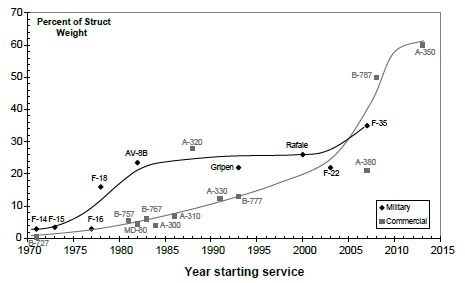
\includegraphics[scale=1.0]{figura/UseOfComposites}
	\legend{Fonte: \cite[p. 6]{kassapoglou2013design}}
\end{figure}

\section{Visão geral}
De acordo com \cite{daniel2006engineering}, os materiais compostos possuem diversas vantagens de utilização em relação aos materiais metálicos como elevada resistência, elevada rigidez, vida longa em fadiga, baixa densidade e alta adaptabilidade em relação a função de utilização pretendida pela estrutura. A superior perfomance estrutural dos materiais compostos se deve basicamente às elevadas resistência e rigidez específicas e à anisotropia do material, visto que devido à esta última característica, o material composto possui diversos graus de liberdade para uma configuração ótima do laminado. No geral, devido ao elevado número de graus de liberdade é possível realizar a otimização do laminado em material composto para diversas restrições de projeto e objetivos, como menor peso estrutural, máxima estabilidade dinâminca e/ou menor custo de fabricação. No entanto, todo o processo requer um confiável banco de dados das propriedades dos materiais, métodos de análises estruturais, técnicas de modelagem e simulações padronizadas e certificadas. Logo, devido às numerosas opções disponíveis, os processos e análises acabam se tornando mais complexas em relação aos materiais convencionais.

Os materiais compostos possuem algumas limitações de uso em relação ao materiais metálicos. Do ponto de vista da micromecânica, as fibras dos materiais compostos possuem uma grande variabilidade nas propriedades de resistência e concentradores de tensão locais reduzem consideravelmente a resistência a tração das estruturas projetadas em materiais compostos. Em relação a macromecânica, a anisotropia do material pode ser utilizada considerada como uma vantagem visto que o comportamento do material pode ser variado, no entando, esta mesma característica faz com que as análises desses materiais sejam muito mais complexas \cite{daniel2006engineering}.

\section{Parâmetros de laminação}


\[
\begin{bmatrix}
    \xi_{11}^2       & x_{12} & x_{13} & \dots & x_{1n} \\
    x_{21}       & x_{22} & x_{23} & \dots & x_{2n} \\
    \hdotsfor{5} \\
    x_{d1}       & x_{d2} & x_{d3} & \dots & x_{dn}
\end{bmatrix}
=
\begin{bmatrix}
    x_{11} & x_{12} & x_{13} & \dots  & x_{1n} \\
    x_{21} & x_{22} & x_{23} & \dots  & x_{2n} \\
    \vdots & \vdots & \vdots & \ddots & \vdots \\
    x_{d1} & x_{d2} & x_{d3} & \dots  & x_{dn}
\end{bmatrix}
\]

\section{Práticas de projeto para materiais compostos}
Esta seção apresenta regras e práticas relevantes utilizadas durante o projeto de estruturas em materiais compostos na indústria aeronáutica.

\subsection{Laminados simétricos}
Os laminados que possuem um sequência	de ângulos das lâminas simétrico em relação ao plano médio, são chamados de laminados simétricos. Conforme descrito por \cite{mil2002handbook} e \cite{niucomposite}, a maior vantagem da utilização de um laminado simétrico é o desacoplamento entre o comportamento de membrana e flexão da estrutura.

Em um laminado simétrico, conforme notação apresentada na \autoref{fig_laminate} e conforme a \autoref{eq_matrixB} matriz [B] do laminado se anula.

\begin{figure}[h]
	\caption{\label{fig_laminate}Notação para espessura do laminado e sequência das lâminas}
  \centering
  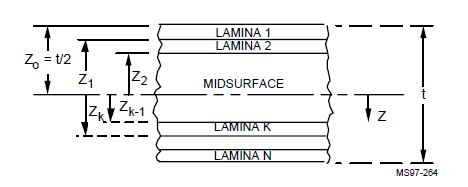
\includegraphics[scale=1.0]{figura/Laminate}
	\legend{Fonte: \cite{mil2002handbook}}
\end{figure}

\begin{equation} \label{eq_matrixB}
B_{ij}
=
\sum_{k=1}^N (\overline{Q}_{ij})_k [z_k^2 - (z_{k-1})^2]
\end{equation}

Sabe- se que $ \overline{Q}_{ij} $ corresponde a rigidez da lâmina. E sabe-se também que a matriz $ B_{ij} $ é a responsável pelo acomplamento entre a reposta no plano e a flexão do laminado. Portanto, conforme \cite{nasa1997guidelines}, quando a matriz $ B_{ij} $ não é zerada, um carregamento no plano induz curvaturas, e momentos de flexão induzem deformações no plano. Nota-se pela \autoref{eq_matrixB} que a matriz $ B_{ij} $ possui termos da coordenada z elevados ao quadrado, portanto, quando o laminado possui simetria geométrica e de materiais em relação ao plano médio, este termo é zerado.

\subsection{Laminados balanceados}
Os laminados balanceados são aqueles em que todas as lâminas, com exceção das de 0$^{\circ}$ e das de 90$^{\circ}$, devem ocorrer em pares de $ +\theta $ e $ -\theta $ acima e abaixo do plano médio do laminado. Para o conjunto de laminados compostos por lâminas com ângulos 0/$\pm$45/90, cada lâmina de +45$^{\circ}$ deve ser acompanhada de um lâmina de -45$^{\circ}$.
Laminados balanceados possuem vantagens similares às vantagens do laminados simétricos. Uma delas é que o acoplamento de membrana entre o comportamento normal e de cisalhamento no plano da estrutura é removido, visto que ambos os coeficientes, $ A_{16} $ e $ A_{26} $, são iguais a zero \cite{nasa1997guidelines}. Este comportamento pode ser explicado observado as equações do carregamento de membrana de um laminado simétrico, \autoref{eq_loadingA}, \autoref{eq_A16} e \autoref{eq_A26}.

\begin{equation} \label{eq_loadingA}
\begin{bmatrix}
    N_{x} \\
    N_{y} \\
    N_{xy} \\
\end{bmatrix}
=
\begin{bmatrix}
    A_{11} & A_{12} & A_{16}\\
    A_{12} & A_{22} & A_{26}\\
    A_{16} & A_{26} & A_{66}\\
\end{bmatrix}
\begin{bmatrix}
    \varepsilon_{x}^o \\
    \varepsilon_{y}^o \\
    \gamma_{xy}^o \\
\end{bmatrix}
\end{equation}

\begin{equation} \label{eq_A16}
A_{16}
=
\sum_{k=1}^N (\overline{Q}_{16})_k t_k
\end{equation}

\begin{equation} \label{eq_A26}
A_{26}
=
\sum_{k=1}^N (\overline{Q}_{26})_k t_k
\end{equation}

Onde

\begin{equation} \label{eq_Q16}
(\overline{Q}_{16})_k
=
({Q}_{11}-{Q}_{12}-2{Q}_{66})_k \sin\theta \cos^3\theta + ({Q}_{11}-{Q}_{22}-2{Q}_{66})_k \sin^3\theta \cos\theta
\end{equation}
\begin{equation} \label{eq_Q26}
(\overline{Q}_{26})_k
=
({Q}_{11}-{Q}_{12}-2{Q}_{66})_k \sin^3\theta \cos\theta + ({Q}_{11}-{Q}_{22}-2{Q}_{66})_k \sin\theta \cos^3\theta
\end{equation}

Sabe- se que $ \overline{Q}_{ij} $ corresponde a rigidez da lâmina e que $ t_k $ corresponde a espessura da lâmina. Nota-se também que ambas as expressões de $ A_{16} $ e $ A_{26} $ contém potências ímpares de $ \sin\theta $ e $ \cos\theta $. Logo lâminas com ângulos de 0$^{\circ}$ e 90$^{\circ}$ não contribuem para os termos de $ A_{16} $ e $ A_{26} $ e estes termos são reduzidos a zero em qualquer laminado balanceado \cite{nasa1997guidelines}.

A \autoref{fig_balancedlaminate} apresenta dois laminados, um desbalanceado, visto que faltam lâminas com -45$^{\circ}$ e um balanceado.

\begin{figure}[ht]
	\caption{\label{fig_balancedlaminate}Laminado desbalanceado e laminado balanceado}
  \centering
  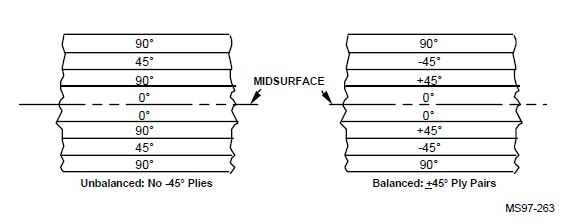
\includegraphics[scale=1.0]{figura/BalancedLaminate}
	\legend{Fonte: \cite{mil2002handbook}}
\end{figure}

Portanto, satisfazendo esta prática de projeto de utilizar somente laminados balanceados, tem-se a seguinte \autoref{eq_result_loadingA} resultante para tensão-deformação

\begin{equation} \label{eq_result_loadingA}
\begin{bmatrix}
    N_{x} \\
    N_{y} \\
    N_{xy} \\
\end{bmatrix}
=
\begin{bmatrix}
    A_{11} & A_{12} & 0\\
    A_{12} & A_{22} & 0\\
    0 & 0 & A_{66}\\
\end{bmatrix}
\begin{bmatrix}
    \varepsilon_{x}^o \\
    \varepsilon_{y}^o \\
    \gamma_{xy}^o \\
\end{bmatrix}
\end{equation}

\subsection{Laminados balanceados}
